\documentclass[14pt]{beamer}
\usepackage[utf8]{inputenc}
\usepackage{amsmath}
\usepackage{amsfonts}
\usepackage{amssymb}
%\usepackage[compat=1.0.0]{tikz-feynman}
\institute{Instituto de Ciencias Nucleares, UNAM}
\author{José Antonio García Hernández}
\title{The profile of non-standard cosmic strings}
%\setbeamercovered{transparent} 
\setbeamertemplate{navigation symbols}{} 
\setbeamertemplate{footline}[frame number]

%Add video
\    usepackage{movie15}
%\usepackage{multimedia}
%\usepackage{media9}

%\usepackage{tikz}
%\logo{} 
%\institute{} 
\date{XV Latin American Symposium on High Energy Physics\\ November 7 2024} 
%\subject{} 
\usepackage{array}
\newcolumntype{C}[1]{>{\centering\arraybackslash}p{#1}@{}}

%\usepackage[]{biblatex}
%\setbeamertemplate{bibliography item}{\insertbiblabel}

\begin{document}


\begin{frame}
\titlepage
\end{frame}



\begin{frame}{Kibble Mechanism}
It is generally assumed that phase transitions occurred in the early universe at the late stages of inflation. These transitions could have formed topological defects. \\~\

Examples:\\
\begin{itemize}
	\item $\pi_0(\mathcal{M}) \neq I \Rightarrow$ Domain wall 
	\item $\pi_1(\mathcal{M}) \neq I\Rightarrow$ Vortex (2d), cosmic strings (3d) 
	\item $\pi_2(\mathcal{M}) \neq I\Rightarrow$ Monopole

\end{itemize}

\end{frame}


\begin{frame}
\centering
%movie15
\includemovie[autoplay]{0.5\textwidth}{0.5\textwidth}{SizingAndSpacing.mp4}
%\movie[poster, height=6.5cm, width=6.5cm]{}{SizingAndSpacing.mp4}
%media9
%\includemedia[width=0.6\linewidth, height=0.45\linewidth, addresource=SizingAndSpacing.mp4, activate=onclick, deactivate=onclick]{Movie}{SizingAndSpacing.mp4}
\end{frame}

\section{Cosmic Strings}
\begin{frame}{Cosmic Strings}
%\begin{tabular}{@{} {2}{C{\linewidth}} }
  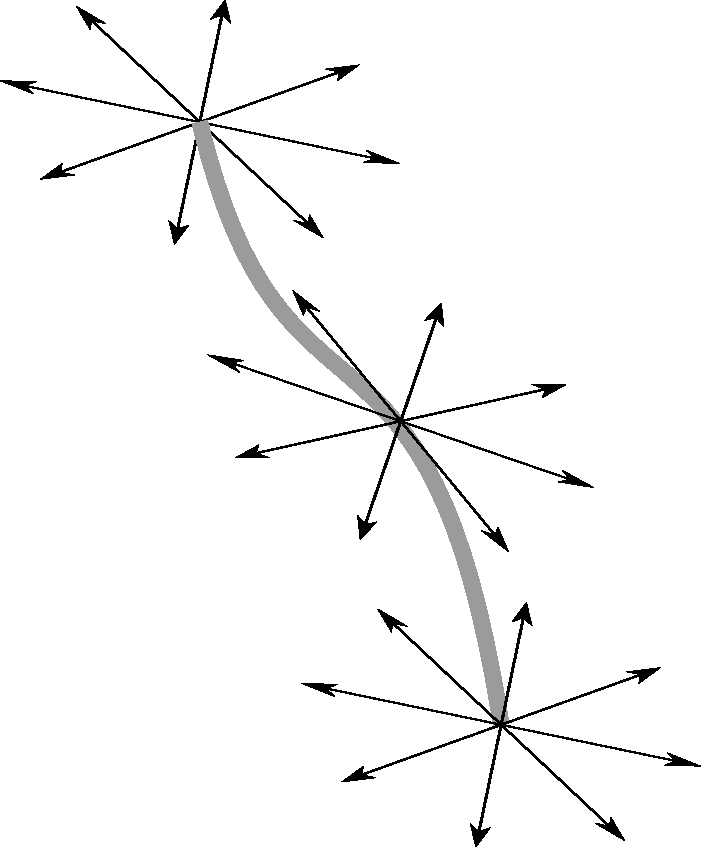
\includegraphics[scale=0.4]{chapters/figures/string.pdf} %\\[\abovecaptionskip]
2-dimensional vortices stacked on top of each other, forming a cosmic string in three dimensions 
%\end{tabular}

\end{frame}



\section{U(1)$_{B-L}$ exact local symmetry}
\begin{frame}{U(1)$_{B-L}$ exact local symmetry}
In the Standard Model U(1)$_{B-L}$ is an \textbf{exact} global symmetry. $B$ baryon number, $L$ lepton number.\\~\

This is strange, an exact symmetry is only natural when it is local.\\~\
\end{frame}

\begin{frame}{Gauge symmetry}
We promote U(1)$_{B-L}$ to a local symmetry and combine it with U$(1)_Y$. \\~\

We introduce a new gauge coupling $h'$ and define a new charge as
	$$Y' \equiv 2hY + \frac{h'}{2}(B-L).$$
We take the gauge group to be U(1)$_{Y'}$ and we call the gauge field $\mathcal{A}_{\mu}$ .\\~\
\end{frame}


\begin{frame}{Gauge Anomaly}
%\begin{tabular}{@{} *{2}{C{\linewidth}} }
  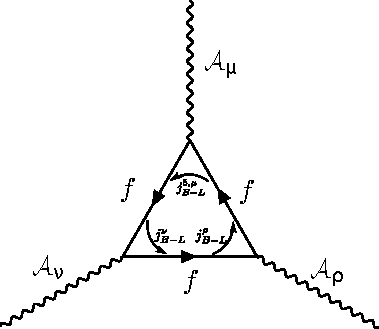
\includegraphics[scale=1]{chapters/figures/triangularanomaly.pdf}% \\[\abovecaptionskip]
In each vertex the quarks of one generation contribute with $B=4$, and leptons with $L=3$. $B-L\neq 0$.
%%\end{tabular}
\end{frame}

\begin{frame}

Gauge anomaly. It is cured by adding a $\nu_R$ ($L=1$) to each generation. \\~\

Since the neutrinos have mass, it is natural to introduce a mechanism to give mass to the neutrinos.
\end{frame}


%\begin{frame}
%We can give mass to the neutrino with a Dirac mass term 
%$$ f_{\nu} \left[\bar{\nu}_R \begin{pmatrix}-\Phi_0 & \Phi_+\end{pmatrix}\begin{pmatrix}
%	\nu_L \\
%	e_L
%\end{pmatrix} + \begin{pmatrix}\bar{\nu}_L & \bar{e}_L\end{pmatrix}
%\begin{pmatrix}
%	-\Phi^*_0 \\
%	\Phi^*_+
%\end{pmatrix}\nu_R\right], $$
%where $f_{\nu}$ is a Yukawa coupling.\\~\
%
%\end{frame}


%\begin{frame}
%Usually we can give mass to the right-handed neutrinos with a Majorana mass term
%$$	M(\bar{\nu}_R+{\nu}^T_RC)(\nu_R+C\bar{\nu}_R^T). $$
%However, in our scenario, this term is forbidden since it breaks the U$(1)_{Y'}$ gauge symmetry.
%\end{frame}


\begin{frame}
To add a mass term solely for $\nu_R$, independently of $\nu_L$, we add a new Higgs field $\chi\in\mathbb{C}$
$$f_{\nu_R} \nu_R^T \chi \nu_R + \text{c.c.},$$
where $f_{\nu_R}$ is a Yukawa coupling. \\~\

To preserve gauge invariance, the field $\chi$ must have a charge $B-L=2$.
\end{frame}

\begin{frame}
We generate the Majorana mass with the Higgs mechanism using the new Higgs field $\chi \in \mathbb{C}$ .\\~\

We denote the vacuum expectation value of $\chi$ as $v'$. \\~\

$\chi$ gives a Majorana mass to the right-handed neutrino $M = f_{\nu_R} v'$.  \\~\

\end{frame}

\begin{frame}

$\chi$ is added to the Lagrangian with the potential
$$V' = \frac{m'^{2}}{2}\chi^*\chi+\frac{\lambda'}{4}(\chi^*\chi)^2.$$ 

It is natural to include  
$$ \frac{\kappa}{2}\Phi^{\dagger}\Phi\chi^*\chi.$$

We assume that $v'\gg v$ and $f_{\nu_R}\simeq O(1)$ in order to give a large mass to the right-handed neutrino.
\end{frame}

\subsection{Lagrangian}
\begin{frame}{Lagrangian}
\begin{eqnarray*} 
\mathcal{L} & = & \frac{1}{2}(D^{\mu}\Phi)^{\dagger}D_{\mu}\Phi - \frac{m^2}{2}\Phi^{\dagger}\Phi - \frac{\lambda}{4}(\Phi^{\dagger}\Phi)^2 -\frac{\lambda}{4}v^4   \nonumber\\
 & & +\frac{1}{2}(D^{\mu} \chi)^*D_{\mu} \chi - \frac{m'^2}{2}\chi^*\chi - \frac{\lambda'}{4}(\chi^* \chi)^2 -\frac{\lambda'}{4}v'^4\nonumber \\ 
 & & -\frac{\kappa}{2}\Phi^\dagger\Phi\chi^*\chi  -\frac{\kappa}{2}v^2v'^2 -\frac{1}{4}\mathcal{F}^{\mu\nu}\mathcal{F}_{\mu\nu}, %+ \frac{1}{4}B_{\mu\nu}B_{\mu\nu}
\end{eqnarray*}

\begin{itemize}
	\item $\Phi = (\phi_+,\phi_0)^{\text{T}} \in \mathbb{C}^2$
	\item $D_{\mu} \Phi = (\partial_{\mu} + ih\mathcal{A}_{\mu})\Phi$
	\item $D_{\mu} \chi = (\partial_{\mu} + ih'\mathcal{A}_{\mu})\chi$
	\item $\mathcal{F}_{\mu\nu}= \partial_{\mu}\mathcal{A}_{\nu}-\partial_{\nu}\mathcal{A}_{\mu}$
\end{itemize}
\end{frame}

\begin{frame}
For the potential to be bounded from below, we need
\begin{equation*}
	\lambda>0, \ \ \ \lambda'>0, \ \ \ \kappa^2 < \lambda \lambda',
\end{equation*}
and for spontaneous symmetry breaking to occur
\begin{eqnarray*}
 m^2 = -\kappa v'^2 - \lambda v^2<0,\\
  m'^2 = -\kappa v^2 - \lambda' v'^2<0.
\end{eqnarray*}

\end{frame}

\begin{frame}{Equations of motion}
\begin{eqnarray*}
	D^{\mu}D_{\mu} \Phi & = & -m^2 \Phi - \lambda (\Phi^{\dagger}\Phi)\Phi - \kappa \Phi \chi^* \chi \\
	D^{\mu}D_{\mu} \chi & = & -m'^2 \chi - \lambda' (\chi^{*}\chi)\chi - \kappa \chi \Phi^{\dagger} \Phi \\
	\partial^{\lambda}\mathcal{F}_{\lambda\nu}  & = & -\frac{ih}{2}\left[ (D_{\nu}\Phi)^{\dagger}\Phi-\Phi^{\dagger}(D_{\nu}\Phi)\right] \\
	& & - \frac{ih'}{2}\left[ (D_{\nu}\chi)^{*}\chi-\chi^{*}(D_{\nu}\chi)\right]
\end{eqnarray*}
\end{frame}

\begin{frame}{Ansatz}
The Lagrangian has a U$(1)_{Y'}$ symmetry which can ``spontaneously break" down to $I$. \\~\

$\mathcal{M} = \text{U}(1)_{Y'}/I=\text{U}(1) \Rightarrow \pi_1(\text{U}(1)) = \mathbb{Z} \Rightarrow$ cosmic strings. \\~\

We only consider the component $\phi_0$ of the Higgs field $\Phi$. Cylindrically symmetric ansatz

\begin{eqnarray*}
	\phi_0(r,\varphi) & = & \phi(r) e^{in\varphi} \\
	\chi(r,\varphi) & = & \xi(r) e^{in'\varphi} \\
	\mathbf{\mathcal{A}}(r) & = & \frac{a(r)}{r} \hat{\varphi}.
\end{eqnarray*}

\end{frame}
\subsection{Equations of motion}
\begin{frame}{Equations of motion}
\begin{eqnarray*}
\partial_r^2 \phi + \frac{1}{r} \partial_r \phi- \frac{\left(n+ha\right)^2}{r^2}\phi- m^2 \phi- \lambda \phi^3-\kappa \phi \xi^2 = 0 \\
\partial_r^2 \xi + \frac{1}{r} \partial_r \xi - \frac{\left(n'+h'a\right)^2}{r^2}\xi -m'^2\xi - \lambda' \xi^3 -\kappa \xi \phi^2 = 0\\
\partial_r^2a -\frac{1}{r}\partial_r a-h(n+ha)\phi^2-h'(n' + h'a )\xi^2 = 0.
\end{eqnarray*}
Boundary conditions
\begin{eqnarray*}
	\phi(0)=0, & \displaystyle\lim_{r\to\infty}\phi(r) = v \\
	 \xi(0)=0, &  \displaystyle\lim_{r\to\infty}\xi(r) = v' \\
	 a(0)=0, & \displaystyle \lim_{r\to\infty}a(r) = -\frac{n}{h}=-\frac{n'}{h'} .
\end{eqnarray*}

\end{frame}

\begin{frame}

Boundary value problem, numerical solutions with the damped Newton method.\\~\

Solutions uniquely defined by inserting $v$, $v'$, $\lambda$, $\lambda'$, $h$, $h'$, $n$ and $n'$.\\~\

We choose $v'\gg v$. \\~\

$v=246$ GeV is used to convert all dim'less variables to physical units. 
We display the profile radius $r$ in units of  
\begin{equation*}
	 v_{\text{dim'less}}\cdot 0.0008\ \text{fm}.
\end{equation*}

\end{frame}

\subsection{Results}


\begin{frame}
%%\begin{tabular}{@{} *{2}{C{\linewidth}} }
  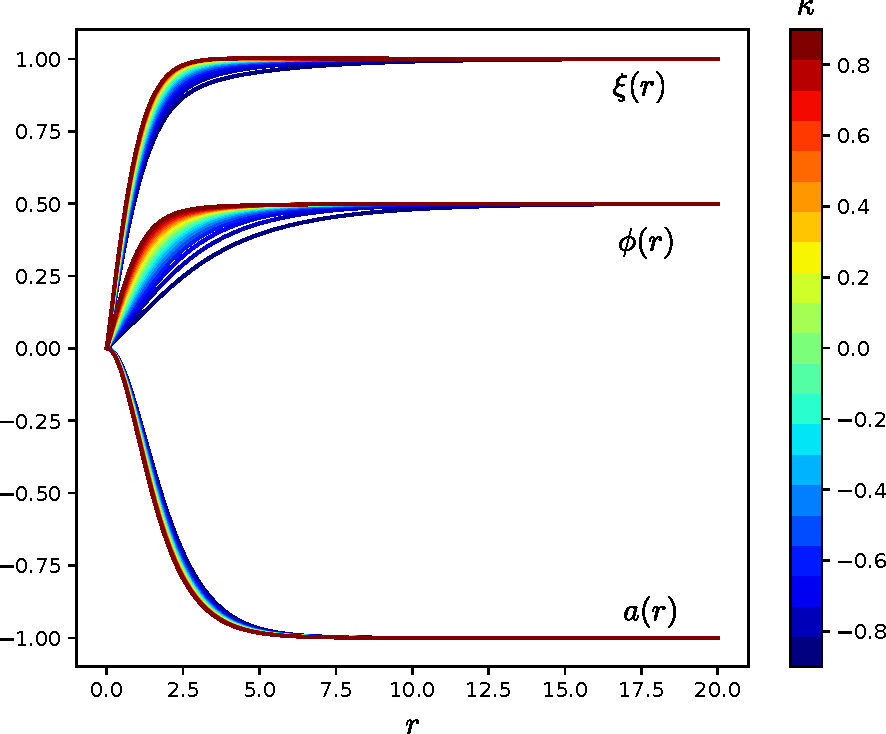
\includegraphics[scale=0.6]{chapters/figures/F0.pdf} %\\[\abovecaptionskip]
$v=0.5$, $v'=1$, $n=n'=h=h'=\lambda=\lambda'=1$.
%%\end{tabular}
\end{frame}

\begin{frame}
%%\begin{tabular}{@{} *{2}{C{\linewidth}} }
  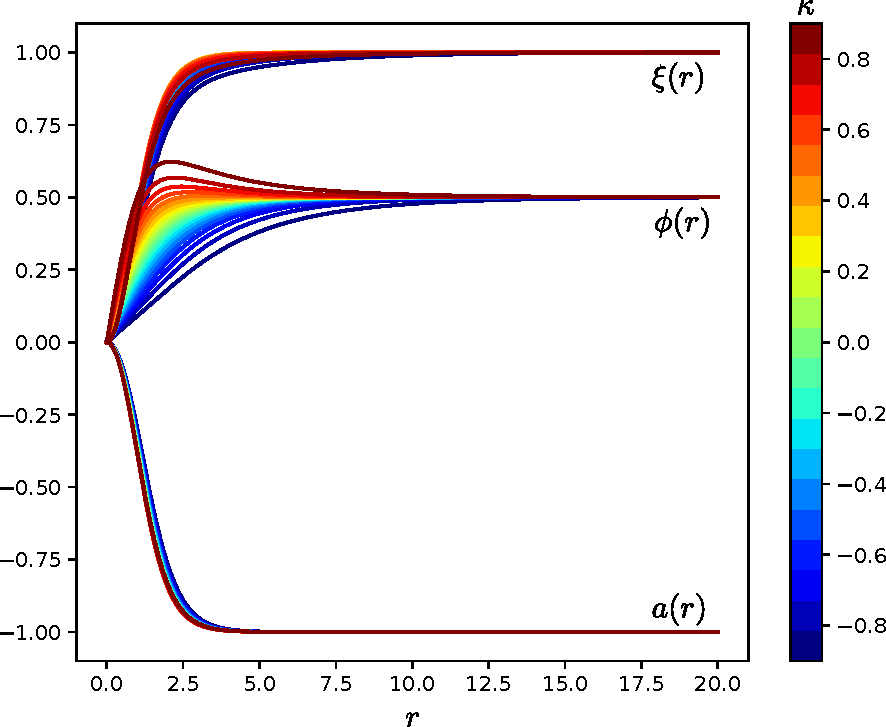
\includegraphics[scale=0.6]{chapters/figures/Figure_1.pdf} %\\[\abovecaptionskip]
$v = 0.5$, $v'=1$, $n=1$, $n'=2$, $h=1$, $h'=2$, $\lambda=\lambda'=1$.
%%\end{tabular}
\end{frame}
%
\begin{frame}
%%\begin{tabular}{@{} *{2}{C{\linewidth}} }
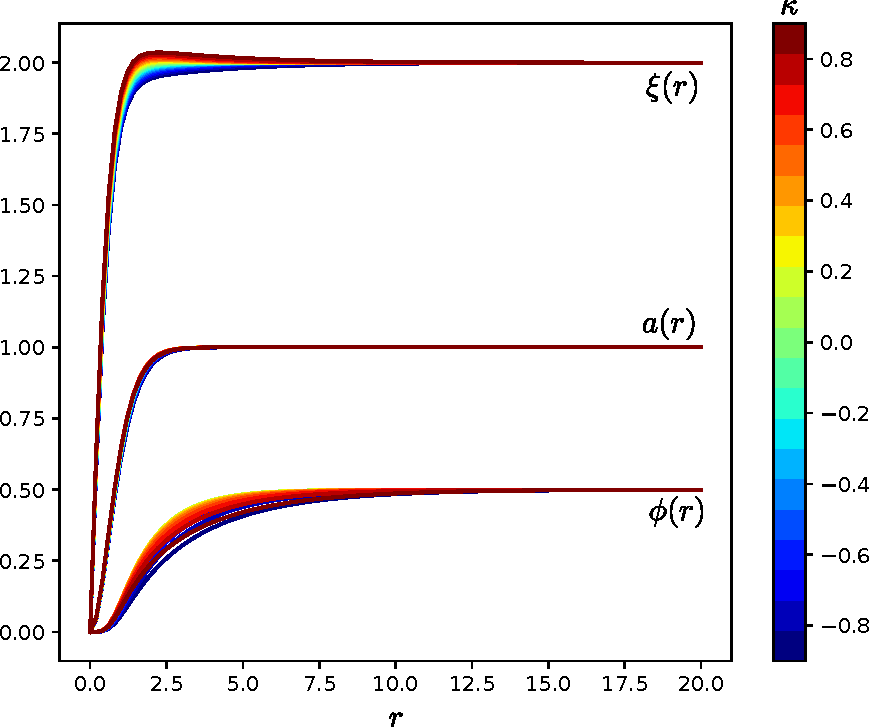
\includegraphics[scale=0.5]{chapters/figures/n-5h5np-1hp1l1lp1v05vp2.pdf} %\\[\abovecaptionskip]
$v = 0.5$, $v'=2$, $n=-5$, $n'=-1$, $h=5$, $h'=1$, $\lambda=\lambda'=1$. This is an example from the SO(10) GUT [Buchm\"uller/Greub/Minkowski, '91].
%%\end{tabular}
\end{frame}

\begin{frame}

%\begin{tabular}{@{} *{2}{C{\linewidth}} }
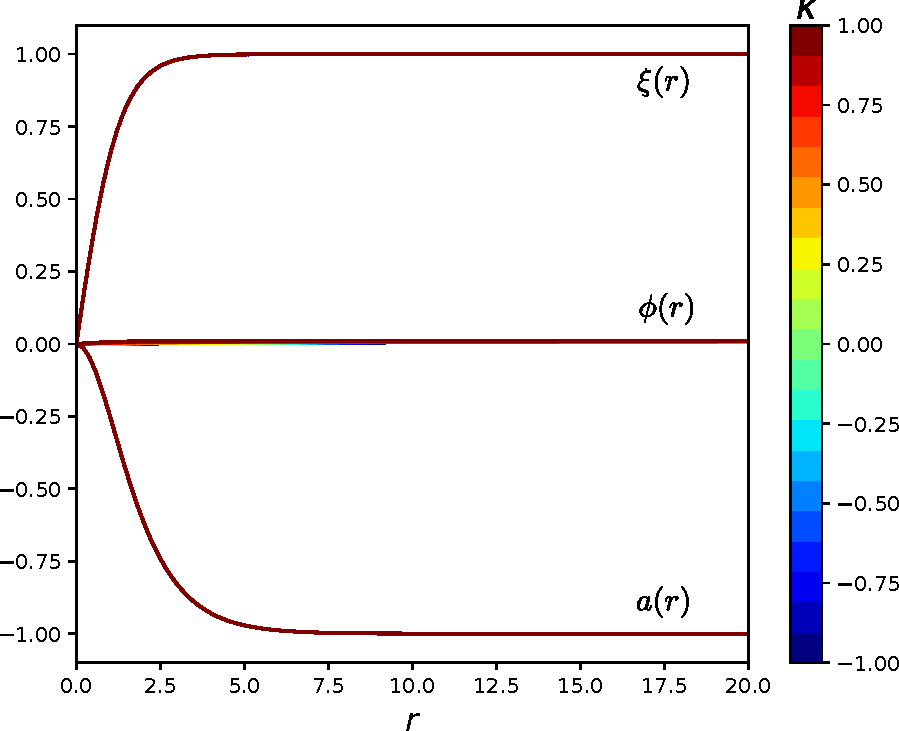
\includegraphics[scale=0.6]{chapters/n1h1np1hp1l1lp1v001vp1edited.pdf}% \\[\abovecaptionskip]
$n = h = n' = h'  = \lambda=\lambda' = 1,\ v =0.01,\ v' = 1 $
%\end{tabular}
\end{frame}

\begin{frame}

%\begin{tabular}{@{} *{2}{C{\linewidth}} }
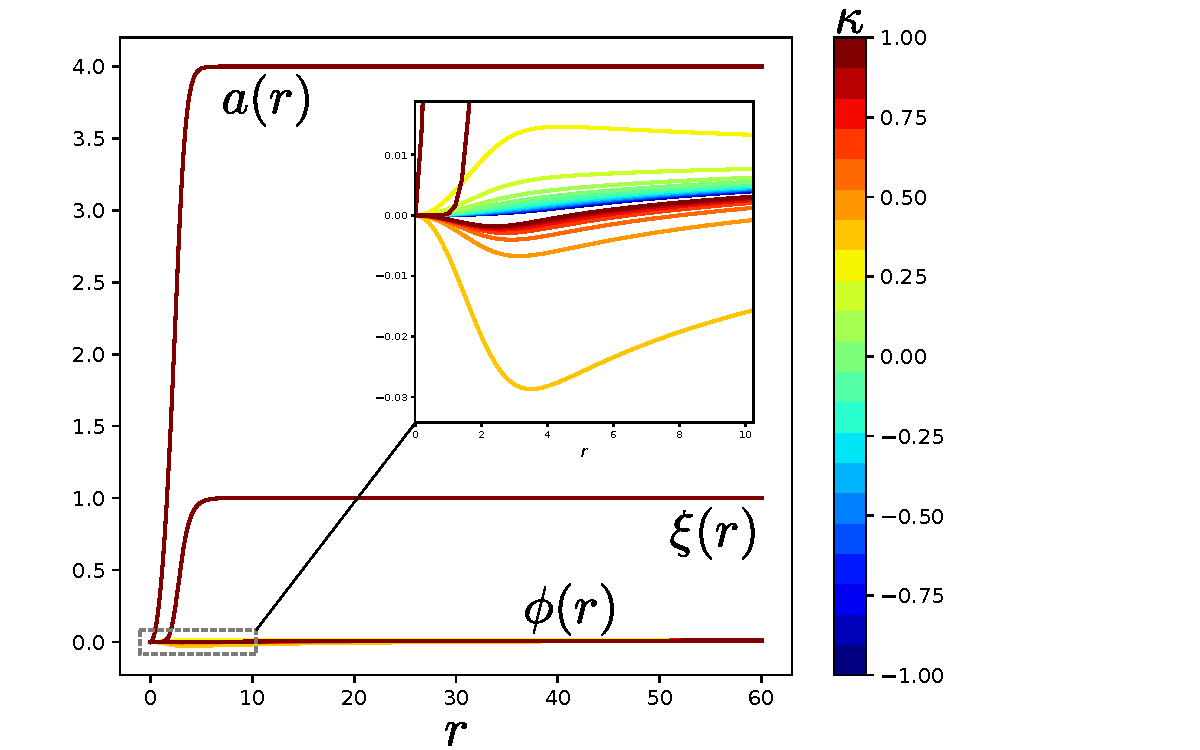
\includegraphics[scale=0.55]{chapters/n-2h05np10hp-25l1lp1v001vp1combined.pdf} %\\[\abovecaptionskip]
\textbf{Coaxial string solution}, cf.\ [Bogomol'nyi, 1975] with $n = -2,\ h =0.5,\ n' = 10,\ h' = -2.5,\  \lambda=1,\ \lambda' = 1,\ v =0.01,\ v' = 1$.
%\end{tabular}
\end{frame}



\begin{frame}
\begin{figure}
	\centering
	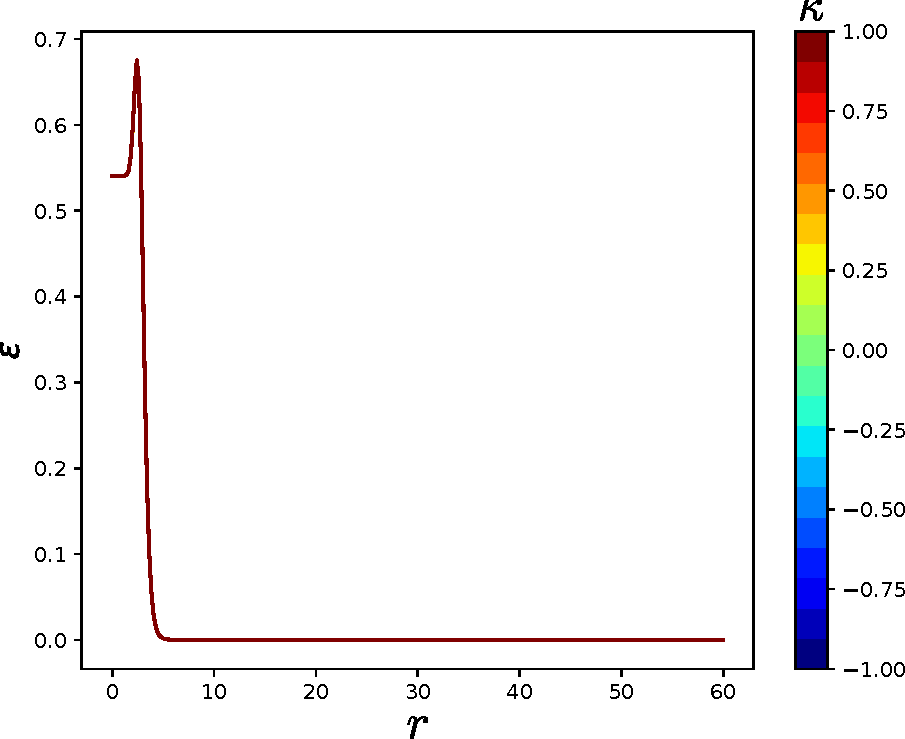
\includegraphics[scale=.5]{chapters/figures/n-2h05np10hp-25l1lp1v001vp1eden.pdf}
	\caption{Energy density, $v = 0.01$, $v'=1$, $n=-2$, $n'=10$, $h=0.5$, $h'=-2.5$, $\lambda=\lambda'=1$, in units of $4.79\times 10^{19}\ \text{GeV}/\text{fm}^3$.}
%	\label{fig:edencoaxial}
\end{figure}
\end{frame}

\begin{frame}
By integrating the energy density we find that the string tension is of the order of
\begin{equation*}
	\mu \sim 10^{10}\ \text{GeV}^2 = 10^{25} \ \frac{\text{kg}}{\text{pc}}.
\end{equation*}
Therefore
\begin{equation*}
	G\mu \sim 10^{-28},
\end{equation*}
where $G = \frac{1}{(1.2\times 10^{19}\ \text{GeV})^2}$.\\~\

The LIGO/Virgo collaboration set constraints to the string tension
\begin{equation*}
		G\mu \lesssim 4\times 10^{-15}.
	\end{equation*}		
\end{frame}

\section{Summary}
\begin{frame}{Summary}
In this BSM model, we added
\begin{itemize}
	\item A new gauge coupling $h'$ 
	\item A right-handed neutrino $\nu_R$
	\item A new Higgs field $\chi\in\mathbb{C}$ \\~\

\end{itemize}

A non-standard type of cosmic strings is possible.\\~\

Overshoot and coaxial string solutions. \\~\
 
At large distances, they do not affect known physics.\\~\


\end{frame}
 
\begin{frame}


Not observed but detectable, in principle. Like gravitational wave detection, gravitational lensing, CMB anisotropies etc. \\~\

No contradictions with SM physics, motivated from the exactness of U$(1)_{B-L}$.
\end{frame}



\end{document}

